\documentclass{article}
\usepackage{hyperref}
\usepackage{graphicx}
\usepackage{lmodern}  % for bold teletype font
\usepackage{amsmath}  % for \hookrightarrow
\usepackage{xcolor}   % for \textcolor
\usepackage{listings}
\lstset{
  basicstyle=\ttfamily,
  columns=fullflexible,
  frame=single,
  breaklines=true,
  postbreak=\mbox{\textcolor{red}{$\hookrightarrow$}\space},
}
\addtolength{\oddsidemargin}{-.875in}
	\addtolength{\evensidemargin}{-.875in}
	\addtolength{\textwidth}{1.75in}

	\addtolength{\topmargin}{-.875in}
	\addtolength{\textheight}{1.75in}
\renewcommand{\baselinestretch}{0.97}
\title{CS-2375 Project: F1DB}
\author {Vidur Kaushik, Gautam Yajaman}

\date{29th October, 2023}

\begin{document}

\maketitle

\noindent
Demo video URL: \url{https://drive.google.com/file/d/1RtXmmR-y6afqfqBGnGSbcdKUcRUov-dn/view?usp=drive_link}

\section{Section 1}
\textbf{Motivation:} Formula 1 is a statistic heavy sport, and it is hard for casual fans to keep up with it if they do not follow it regularly. Drivers retire, teams fall out of competitiveness,and other teams rise to the top. Using our database, anyone can keep up with the sport at their own convenience, as well as access the data from previous seasons. The frontend we have made is a clean interface that is easy to use and provides all the information fans will need to keep up with the sport, including pages for every race, driver, team and circuit. The backend of the site can be updated whenever needed, ensuring that the database is up to date.\\

\noindent
Below is an ER diagram of our database generated by the software DBVisualiser. This neatly outlines how each relations are connected to one another:

\begin{center}
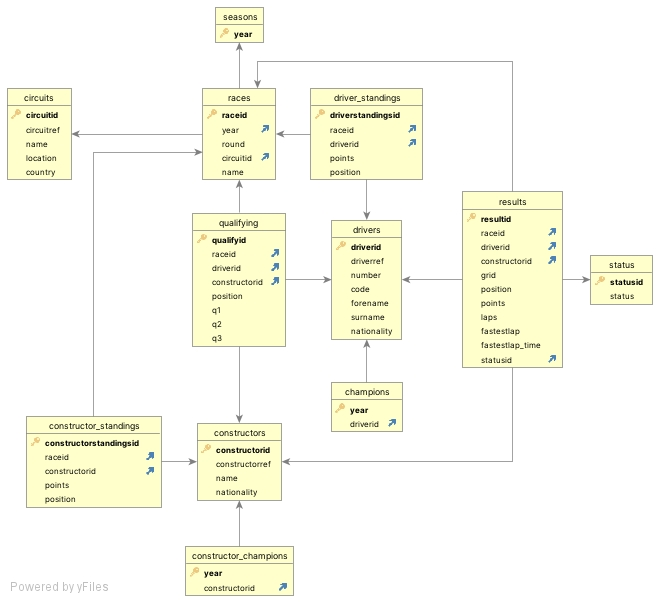
\includegraphics[scale=0.5]{ERDIAG.jpg}
\end{center}

\newpage
\section{Section 2}
\begin{enumerate}
	\item \url{https://www.kaggle.com/datasets/rohanrao/formula-1-world-championship-1950-2020}
	\item The data was readymade.
	\item We removed some \texttt{.csv} files that were not relevant to the outcome of our project. Also we removed some columns from the data that were not useful. This did not affect the final product. We also added two new files to make querying easier.
	\item The metadata is given below:
	
	\begin{tabular}{|c|c|}
		\hline
		\textbf{Name}&\textbf{Tuple Count}\\
		\hline
		\hline
		champions&73\\
		\hline
		circuits&77\\
		\hline
		constructor\_champions&65\\
		\hline
		constructor\_standings&13051\\
		\hline
		constructors&211\\
		\hline
		driver\_standings&34124\\
		\hline
		drivers&857\\
		\hline
		qualifying&9815\\
		\hline
		races&1101\\
		\hline
		results&26080\\
		\hline
		seasons&74\\
		\hline
		status&139\\
		\hline
	\end{tabular}

	The data takes around 6 seconds to import into PostgreSQL. The uncleaned data has a size of 19.6 MB. The final data we used was around 2 MB.
\end{enumerate}
\section{Section 3}
\begin{enumerate}
	\item User's view of the system (note that the user will have a navigation bar with "Home", "Drivers", "Teams", "Circuits", "Seasons" and "Records"):
	\begin{itemize}
		\item \textbf{Home Page:} This has the ten most recent races, the circuit it took place at and the country. Both the race and circuit are clickable, and take you to their respective pages.
		\item \textbf{Drivers:} This has a list of drivers that took part in the most recent race, along with their teams. At the bottom of the page there is a button that takes you to the "All Drivers" page.
		\begin{itemize}
			\item \textbf{All Drivers:} This has a list of all drivers. At the top, there is a search box where you can search for drivers by their name. This takes you to the search results page.
			\item \textbf{Search Results:} This has a list of all drivers that match the search query.
		\end{itemize}
		\item \textbf{Teams:} This has a list of teams that took part in the most recent race. At the bottom of the page there is a button that takes you to the "All Teams" page.
		\begin{itemize}
			\item \textbf{All Teams:} This has a list of all teams. At the top, there is a search box where you can search for teams by their name. This takes you to the search results page.
			\item \textbf{Search Results:} This has a list of all teams that match the search query.
		\end{itemize}
		\item \textbf{Driver Profile:} Any time the user clicks on a driver's name, it takes them to a driver profile which has the drivers stats (wins, podiums, career points, race starts, most recent team, championships). This page also lists all the teammates of the driver, and the average gap in qualifying laptime to that teammate. At the bottom of the page, there is a button that takes the user to page of all of the driver's career results, in a similar fashion to how the homepage is configured.
		\item \textbf{Team Profile:} Any time the user clicks on a team's name, it takes them to a team profile which has the teams stats (wins, podiums, career points, race starts, championships).
		\item \textbf{Seasons:} A page with every season that has happened. Each season is clickable and takes the user to a season page. Each season page has three tables: one with the final driver's championship standings, one with the final constructor's standings and a list of all the races that happened that season.
		\item \textbf{Circuits:} A page with every circuit. Each circuit is clickable and takes the user to a circuit page. Each circuit page has a graph with laptime over the years for all the qualifying sessions that have happened at that circuit (the dataset is limited to 1994 onwards for qualifying times). It also has the most successful teams and drivers at that circuit.
		\item \textbf{Records:} A page with tables (for both teams and drivers) of most wins, most pole positions and most championships. Each of these tables has a link at the bottom that takes the user to a page with the full list.
	\end{itemize}

	\item System view:

	Special functionality:
	\begin{itemize}
		\item \textbf{Normalised Career Points:} Formula 1 has used many different points scoring systems over the years. In 2000, a win gave drivers 10 points, but in 2022, a win gave drivers 25 points. Hence total points is a useless metric to judge a driver's career. This is why we have added a normalised points score. This query filters filters the results relation by driverid, and then computes the total number of points based on finishing position:
		
		\begin{tabular}{|c|c|}
			\hline
			\textbf{Position} & \textbf{Score}\\
			\hline
			1st & 25\\
			2nd & 18\\
			3rd & 15\\
			4th & 12\\
			5th & 10\\
			6th & 8\\
			7th & 6\\
			8th & 4\\
			9th & 2\\
			10th & 1\\
			Below 10th & 0\\
			\hline
		\end{tabular}

		\item \textbf{Gap To Teammate:} Since Formula 1 has cars that are not equal, it is hard to judge a driver's raw speed. The only metric for this is the gap to their teammates in terms of laptime. Hence we added a section on every driver's profile where the average gap to each of their teammates is shown to the user. This gap is computed by taking the best qualifying time of both the drivers in races where they were in the same team, subtracting them, and then computing the average of all these values.
	\end{itemize}

	List of all queries fired:

	\textbf{Home}:\\
        \begin{lstlisting}[language=SQL]
SELECT r.year, r.name as race, c.name as circuit, c.country, r.raceid, 
c.circuitid
FROM races as r, results re, circuits c
WHERE r.raceid = re.raceid AND c.circuitid = r.circuitid
GROUP BY (race, c.name, c.country, r.year, r.round, r.raceid, c.circuitid)
ORDER BY r.year DESC, r.round DESC
LIMIT 10;
\end{lstlisting}\vspace{6mm}


\textbf{Drivers:}
\begin{lstlisting}[language=SQL]
WITH latest_race as (SELECT r.raceid FROM races as r, results re WHERE r.raceid = re.raceid ORDER BY r.year DESC, r.round DESC LIMIT 1) SELECT d.driverid, d.forename||' '||d.surname as driver, c.constructorid, c.name as constructor FROM results r, constructors c, drivers d WHERE r.raceid = (SELECT * FROM latest_race) AND c.constructorid = r.constructorid AND d.driverid = r.driverid ORDER BY r.constructorid

SELECT d.driverid, d.forename||' '||d.surname as name FROM drivers d ORDER BY name ASC

SELECT forename||' '||surname FROM drivers WHERE driverid = $1

SELECT(SELECT COUNT(*) FROM results r JOIN drivers d ON r.driverId = d.driverId WHERE d.driverid = $1 AND r.position = 1) AS number_of_wins, (SELECT COUNT(*) FROM results r JOIN drivers d ON r.driverId = d.driverId WHERE d.driverid = $1 AND r.position IN (1, 2, 3)) AS number_of_podiums, (SELECT COUNT(*) FROM results r JOIN drivers d ON r.driverId = d.driverId WHERE d.driverid = $1 AND r.grid = 1) AS number_of_pole_positions, (SELECT COALESCE(SUM(r.points), 0) FROM results r JOIN drivers d ON r.driverId = d.driverId WHERE d.driverid = $1) AS number_of_points, (SELECT SUM(CASE WHEN r.position = 1 THEN 25 WHEN r.position = 2 THEN 18 WHEN r.position = 3 THEN 15 WHEN r.position = 4 THEN 12 WHEN r.position = 5 THEN 10 WHEN r.position = 6 THEN 8 WHEN r.position = 7 THEN 6 WHEN r.position = 8 THEN 4 WHEN r.position = 9 THEN 2 WHEN r.position = 10 THEN 1 ELSE 0 END) AS total_normalised_points FROM results r JOIN drivers d ON r.driverId = d.driverId WHERE d.driverid = $1) AS number_of_points_normalised, (SELECT COUNT(*) FROM results r JOIN drivers d ON r.driverId = d.driverId WHERE d.driverid = $1) AS number_of_race_starts, (SELECT c.name FROM results AS r, drivers as d, races as ra, constructors as c WHERE r.driverid = d.driverid AND d.driverid = $1 AND r.raceid = ra.raceid AND c.constructorid = r.constructorid GROUP BY (ra.year, ra.round,d.driverid, c.constructorid, c.name) ORDER BY ra.year DESC, ra.round DESC LIMIT 1) AS team, (SELECT COUNT(*) FROM champions C JOIN drivers d ON d.driverId = c.driverId WHERE d.driverid = $1) AS number_of_championships, (SELECT c.constructorid FROM results AS r, drivers as d, races as ra, constructors as c WHERE r.driverid = d.driverid AND d.driverid = $1 AND r.raceid = ra.raceid AND c.constructorid = r.constructorid GROUP BY (ra.year, ra.round,d.driverid, c.constructorid, c.name) ORDER BY ra.year DESC, ra.round DESC LIMIT 1) as teamid;

WITH GivenDriverRaces AS (SELECT r.raceId, r.constructorId,q1, q2, q3 FROM results r JOIN qualifying q ON r.raceId = q.raceId AND r.driverId = q.driverId JOIN drivers d ON r.driverId = d.driverId WHERE d.driverid = $1),TeammateRaces AS (SELECT r.raceId, r.constructorId, r.driverId,q1, q2, q3 FROM results r JOIN qualifying q ON r.raceId = q.raceId AND r.driverId = q.driverId WHERE EXISTS (SELECT 1 FROM GivenDriverRaces gdr WHERE gdr.raceId = r.raceId AND gdr.constructorId = r.constructorId)) SELECT d.driverid, d.forename || ' ' || d.surname AS teammate_name,AVG(LEAST(g.q1, COALESCE(g.q2, g.q1), COALESCE(g.q3, g.q1)) - LEAST(t.q1, COALESCE(t.q2, t.q1), COALESCE(t.q3, t.q1))) AS avg_qualifying_gap FROM GivenDriverRaces g JOIN TeammateRaces t ON g.raceId = t.raceId AND g.constructorId = t.constructorId JOIN drivers d ON t.driverId = d.driverId WHERE d.driverid != $1 GROUP BY d.driverId;

SELECT DISTINCT d2.driverid, d2.forename || ' ' || d2.surname AS teammate_name, 'NO DATA' FROM results r1 JOIN results r2 ON r1.raceId = r2.raceId AND r1.constructorId = r2.constructorId AND r1.driverId != r2.driverId JOIN drivers d2 ON r2.driverId = d2.driverId WHERE r1.driverId = $1 ORDER BY d2.driverid

SELECT ra.raceid, ra.year, ra.name AS race, CASE WHEN r.position IS NULL AND (r.statusid = 81 OR r.statusid = 97) THEN '-' WHEN r.position IS NULL THEN 'NC' ELSE CAST(r.position AS VARCHAR) END AS position, CASE WHEN r.statusId = 81 OR r.statusid = 97 THEN 'DNQ' WHEN r.statusId != 1 THEN 'DNF' ELSE '' END AS status FROM results r JOIN races ra ON r.raceId = ra.raceId JOIN drivers d ON r.driverId = d.driverId LEFT JOIN status s ON r.statusId = s.statusId WHERE d.driverid=$1 ORDER BY ra.year ASC, ra.round ASC;
\end{lstlisting}\vspace{6mm}

\textbf{Teams:}\\

\begin{lstlisting}[language=SQL]
    WITH latest_race as (SELECT r.raceid FROM races as r, results re WHERE r.raceid = re.raceid  ORDER BY r.year DESC, r.round DESC LIMIT 1) SELECT r.constructorid, c.name as constructor FROM results r, constructors c WHERE r.raceid = (SELECT * FROM latest_race) AND c.constructorid = r.constructorid GROUP BY(constructor,r.constructorid) ORDER BY r.constructorid

    SELECT c.constructorid, c.name as name FROM constructors c ORDER BY name ASC

    SELECT name FROM constructors WHERE constructorid = $1

    SELECT(SELECT COUNT(*) FROM results r JOIN constructors c ON r.constructorId = c.constructorId WHERE c.constructorid = $1 AND r.position = 1) AS number_of_wins,(SELECT COUNT(*) FROM results r JOIN constructors c ON r.constructorId = c.constructorId WHERE c.constructorid = $1 AND r.position IN (1, 2, 3)) AS number_of_podiums, (SELECT COUNT(*) FROM results r JOIN constructors c ON r.constructorId = c.constructorId WHERE c.constructorid = $1 AND r.grid = 1) AS number_of_pole_positions, (SELECT COALESCE(SUM(r.points), 0) FROM results r JOIN constructors c ON r.constructorId = c.constructorId WHERE c.constructorid = $1) AS number_of_points,(SELECT COUNT(DISTINCT r.raceId) FROM results r JOIN constructors c ON r.constructorId = c.constructorId WHERE c.constructorid = $1) AS number_of_race_entries;

    SELECT COUNT(*) as champion_count FROM constructor_champions WHERE constructorid = $1;
\end{lstlisting}\vspace{6mm}

\textbf{Seasons}\\

\begin{lstlisting}[language=SQL]
    SELECT * FROM seasons ORDER BY year DESC

    WITH RaceResults AS (SELECT r.raceId, r.year, r.round FROM races r JOIN seasons s ON r.year = s.year WHERE s.year = $1 ORDER BY r.year DESC, r.round DESC LIMIT 1) SELECT ds.driverid, ds.position, d.forename||' '||d.surname as name, ds.points as points FROM driver_standings ds, drivers d, RaceResults rr WHERE ds.raceId = rr.raceId and d.driverid = ds.driverid ORDER BY position ASC;

    WITH RaceResults AS (SELECT r.raceId, r.year, r.round FROM races r JOIN seasons s ON r.year = s.year WHERE s.year = $1 ORDER BY r.year DESC, r.round DESC LIMIT 1) SELECT cs.constructorid, cs.position, c.name as name, cs.points as points FROM constructor_standings cs, constructors c, RaceResults rr WHERE cs.raceId = rr.raceId and c.constructorid = cs.constructorid ORDER BY position ASC;

    SELECT r.round, r.year, r.name as race, c.name as circuit, c.country, r.raceid, c.circuitid FROM races as r, results re, circuits c WHERE r.raceid = re.raceid AND c.circuitid = r.circuitid AND r.year = $1 GROUP BY (race, c.name, c.country, r.year, r.round,r.raceid,c.circuitid) ORDER BY r.round ASC;
\end{lstlisting}\vspace{6mm}

\newpage
\textbf{Circuits}\\

\begin{lstlisting}[language=SQL]
    SELECT c.circuitid, c.name, c.country FROM circuits c, races r GROUP BY (c.circuitid, c.name,c.country) ORDER BY name ASC;

    SELECT name, location, country from circuits WHERE circuitid = $1

    SELECT r.year, MIN(LEAST(q.q1, COALESCE(q.q2, q.q1), COALESCE(q.q3, COALESCE(q.q2, q.q1)))) AS fastest_time FROM qualifying q JOIN races r ON q.raceId = r.raceId JOIN circuits c ON r.circuitId = c.circuitId WHERE c.circuitid = $1 AND q.position = 1 GROUP BY r.year ORDER BY r.year ASC;

    SELECT d.driverid, d.forename||' '||d.surname as drivername,COUNT(*) as number_of_wins FROM results r JOIN races ra ON r.raceId = ra.raceId JOIN circuits ci ON ra.circuitId = ci.circuitId JOIN drivers d ON r.driverId = d.driverId WHERE ci.circuitid = $1 AND r.position = 1 GROUP BY d.driverId, drivername ORDER BY number_of_wins DESC, drivername LIMIT 5;

    SELECT c.constructorid, c.name as constructorname,COUNT(*) as number_of_wins FROM results r JOIN races ra ON r.raceId = ra.raceId JOIN circuits ci ON ra.circuitId = ci.circuitId JOIN constructors c ON r.constructorId = c.constructorId WHERE ci.circuitid = $1 AND r.position = 1 GROUP BY c.constructorId, constructorname ORDER BY number_of_wins DESC, constructorname LIMIT 5;
\end{lstlisting}\vspace{6mm}


\textbf{Records}\\

\begin{lstlisting}[language=SQL]
    SELECT d.driverId, CONCAT(d.forename, ' ', d.surname) AS driver_name, COUNT(c.year) as championship_count FROM champions c JOIN drivers d ON c.driverId = d.driverId GROUP BY d.driverId, driver_name ORDER BY championship_count DESC LIMIT 5;

    SELECT d.driverId, CONCAT(d.forename, ' ', d.surname) AS driver_name, COUNT(r.position) AS wins FROM drivers d JOIN results r ON d.driverId = r.driverId WHERE r.position = 1 GROUP BY d.driverId, driver_name HAVING COUNT(r.position) >= 1 ORDER BY wins DESC LIMIT 5;

    SELECT d.driverId, CONCAT(d.forename, ' ', d.surname) AS driver_name, COUNT(r.grid) AS pole_positions_count FROM drivers d JOIN results r ON d.driverId = r.driverId WHERE r.grid = 1 GROUP BY d.driverId HAVING COUNT(r.grid) >= 1 ORDER BY pole_positions_count DESC LIMIT 5;

    SELECT c.constructorid, c.name AS constructor_name, COUNT(cc.year) AS championship_count FROM constructor_champions cc JOIN constructors c ON cc.constructorid = c.constructorid GROUP BY c.name,c.constructorid ORDER BY championship_count DESC LIMIT 5;

    SELECT d.constructorid, d.name as name, COUNT(r.position) AS wins FROM constructors d JOIN results r ON d.constructorId = r.constructorId WHERE r.position = 1 GROUP BY d.constructorId, name HAVING COUNT(r.position) >= 1 ORDER BY wins DESC LIMIT 5;

    SELECT d.constructorid, d.name as name, COUNT(r.grid) AS poles FROM constructors d JOIN results r ON d.constructorId = r.constructorId WHERE r.grid = 1 GROUP BY d.constructorId, name HAVING COUNT(r.grid) >= 1 ORDER BY poles DESC LIMIT 5;

    SELECT d.driverId, CONCAT(d.forename, ' ', d.surname) AS driver_name, COUNT(c.year) as championship_count FROM champions c JOIN drivers d ON c.driverId = d.driverId GROUP BY d.driverId, driver_name ORDER BY championship_count DESC;

    SELECT c.constructorid, c.name AS constructor_name, COUNT(cc.year) AS championship_count FROM constructor_champions cc JOIN constructors c ON cc.constructorid = c.constructorid GROUP BY c.name,c.constructorid ORDER BY championship_count DESC;

    SELECT d.driverId, CONCAT(d.forename, ' ', d.surname) AS driver_name, COUNT(r.position) AS wins FROM drivers d JOIN results r ON d.driverId = r.driverId WHERE r.position = 1 GROUP BY d.driverId, driver_name HAVING COUNT(r.position) >= 1 ORDER BY wins DESC;

    SELECT d.constructorid, d.name as name, COUNT(r.position) AS wins FROM constructors d JOIN results r ON d.constructorId = r.constructorId WHERE r.position = 1 GROUP BY d.constructorId, name HAVING COUNT(r.position) >= 1 ORDER BY wins DESC;

    SELECT d.driverId, CONCAT(d.forename, ' ', d.surname) AS driver_name, COUNT(r.grid) AS pole_positions_count FROM drivers d JOIN results r ON d.driverId = r.driverId WHERE r.grid = 1 GROUP BY d.driverId HAVING COUNT(r.grid) >= 1 ORDER BY pole_positions_count DESC;

    SELECT d.constructorid, d.name as name, COUNT(r.grid) AS poles FROM constructors d JOIN results r ON d.constructorId = r.constructorId WHERE r.grid = 1 GROUP BY d.constructorId, name HAVING COUNT(r.grid) >= 1 ORDER BY poles DESC;
\end{lstlisting}\vspace{6mm}

\textbf{Races}\\

\begin{lstlisting}[language=SQL]
    SELECT races.year, races.name from races WHERE races.raceid = $1

    SELECT COALESCE(CAST(r.position as varchar),'NC'), d.forename||' '||d.surname, d.driverid, c.name AS constructor_name, c.constructorid, r.points FROM results r JOIN races ra ON r.raceId = ra.raceId JOIN drivers d ON r.driverId = d.driverId JOIN constructors c ON r.constructorId = c.constructorId WHERE ra.raceid = $1 ORDER BY r.position ASC;

    WITH RaceResults AS (SELECT r.raceId, r.year, r.round FROM races r JOIN seasons s ON r.year = s.year WHERE r.raceid = $1) SELECT d.driverid, ds.position, d.forename||' '||d.surname as fullname, ds.points as ppoints, c.constructorid, c.name FROM driver_standings ds, drivers d, RaceResults rr, results re, races r,constructors c WHERE ds.raceId = rr.raceId AND d.driverid = ds.driverid AND c.constructorid = re.constructorid AND ds.driverid = re.driverid AND r.raceid = rr.raceid AND r.raceid = re.raceid GROUP BY (d.driverid, ds.position, fullname, ppoints, c.constructorid, c.name) ORDER BY position ASC;

    WITH RaceResults AS (SELECT r.raceId, r.year, r.round FROM races r JOIN seasons s ON r.year = s.year WHERE r.raceid = $1) SELECT d.constructorid, ds.position, d.name as name, ds.points as points FROM constructor_standings ds, constructors d, RaceResults rr WHERE ds.raceId = rr.raceId and d.constructorid = ds.constructorid ORDER BY position ASC;
	\end{lstlisting}

	\item List of tested queries:
	
		\begin{tabular}{|c|c|c|c|}
		\hline
		1 &drivers/driverid            & driverid                              & 0.144s                       \\
		\hline
		2 &teams/teamid                    & teamid                                & 0.040s                       \\
		\hline
		3 &drivers/driverid 2              & driverid                              & 0.056s                       \\
		\hline
		4 &seasons/year                    & year                                  & 0.042s                       \\
		\hline
		5 &season/year 2                   & year                                  & 0.038s                       \\
		\hline
		6 &circuits/circuitid times        & circuitid                             & 0.044s \\
		\hline
		\end{tabular}

\end{enumerate}

\end{document}